
\title{
    COMS4030A Project-- Report \\
    Investigative Analysis of Heart Disease Diagnosis
    }
\author{
    Shameel Nkosi, 1814731, Coms Hons \\
    Molefe Molefe, 1858893, Coms Hons \\
    Siraj Motaung, 1390537, BDA Hons\\
    }

\maketitle 
%\thispagestyle{empty}
\pagestyle{fancy}
\fancyhf{}
\fancyhead[R]{\thepage}
\fancyhead[L]{COMS4030A Adaptive Computation and Machine Learning - Project}
%\vskip 3mm 
%\pagenumbering{roman}
%\newpage
\pagenumbering{roman} 

\newpage
\tableofcontents

\newpage
\listoffigures

\newpage
\vspace*{\fill}
\begin{abstract}
    \begin{center}
        Everything that gets damaged can reach a point of "beyond repairs," the heart is one of the things you do not wish for it to get to such a stage. Knowing beforehand that you are likely to get heart diseases in the future can help reduce the impact through taking early preventative measures. One way of finding out the likelihood of a person having a heart disease is to have a model that can accurately and intelligently tell you whether you are likely to have heart disease or not. In this report, we discuss the models we built that can aid in solving the problem of telling whether a person has or is likely to have heart diseases. We also discuss their implementations, performances, optimizations, and many more. 
    \end{center}
\end{abstract}
\vspace*{\fill}
\addcontentsline{toc}{section}{Abstact}
\newpage
\pagenumbering{arabic}

\section{Introduction}
Human beings make more sound decisions if they have experience in whatever they are trying to make decisions upon. The best way for one to gain experience is to learn. We aim to teach a computer/model to make decisions based on what it learns from the data we feed it. There are many different techniques we can use to approach the solution to our problem. Each of these techniques has its pros and cons. Below we discuss the technique we employed and reasons as to why we've chosen this particular technique.

Remember that the aim is to whether a person is most likely to have heart diseases or not. We are therefore dealing with a problem whose solution gives a "yes" or "no". In machine learning, this is popularly known as binary classification.  

\subsection{Machine Learning technique and datasets}
\subsubsection{Technique}
Probability theory is a study that involves the likelihood of events occurring. Logistic regression is a machine learning technique that gives a probability of an event taking place. Probabilities allow us to make decisions while acknowledging that we could be making a bad decision though the decision taken at that time seems to be the best. We have chosen logistic regression because it appropriately spits out values of 1's for patients with heart diseases and 0's otherwise. Logistic regression is less sensitive to outliers as compared to other techniques we could have employed. It is relatively straightforward to train and is capable of giving good accuracy scores.

\subsubsection{Datasets}
A machine learning algorithm learns to make decisions based on the data you feed it. The more data the algorithm sees, the more accurate its decisions become. The dataset we used in our project is a combination of four datasets collected from the \href{https://archive.ics.uci.edu/ml/datasets/heart+disease}{UCI website}. The four data sets combined into one have been collected from Cleveland, Hungary, Switzerland, and the VA Long Beach. The dataset has 13 features, namely:
\begin{itemize}
    \item Age in years
    \item sex/gender
    \item type of chest pains
    \item Serum cholestoral in mg/dl
    \item Resting blood pressure
    \item Maximum heart rate achieved
    \item Exercise induced Angina
    \item whether fasting blood sugar is greater than 120 mg
    \item Electrocardiographical Results
    \item ST Depression Induced by Exercise Relative to rest
    \item Number of Major Vessels (0-3) colored by flourosopy
    \item The Slope of the Peak Exercise of ST Segment
    \item \textbf{Target:} whether a patient has a heart disease or not.
\end{itemize}
In the subsequent chapter, we discuss data preparation, data handling, preprocessing, data standardization, and data visualizations.




\newpage
\section{Implementation and Results}
\subsection{data handling}
Data handling is arguable the most important part of building a machine learning algorithm that produces the best accuracy possible. For us to learn machine learning, it had to be well presented and well documented. Similarly, for a machine to learn, data needs to be well presented and it needs to be complete. There are four important parts of data handling worth mentioning, these are: 
\begin{itemize}
    \item \textbf{Dealing with duplicate values: }\textit{Duplicate values} may cause our model to be biased against data that doesn't have duplicate instances. To best train our model, we handle this issue by dropping all \textit{duplicate values}, leaving only one instance of it.
    \item \textbf{Missing Values: }Missing values is the most common defect found in a lot of datasets. Missing values may be a result of a recording error, or maybe the respondent did not know the answer to that specific question, or any other reason not mentioned here. In our project, we deal with missing values in three different ways, namely:
        \begin{itemize}
            \item \textbf{Drop missing values: }Delete the rows that have missing values.
            \item \textbf{Replace with Mode/Mean: }In the case of replacement with mode, replace the missing values with data points that appear the most in that particular column. In the case of replacement by mean, replace the missing values with the average of all values that are not missing in that particular column. In our implementation, we only used replacement by mode. 
            \item \textbf{Learn missing values: }Here we resort to other machine learning algorithms to predict what the missing values would be. We make use of unsupervised learning methods to learn the missing values.
        
        \end{itemize}
        In our project, we generated three different datasets from the above forms dealing with missing values. We then run our models on all these datasets to see which method gives the best accuracy.
    \item \textbf{Data standardization: }Data standardization is the rescaling of the values in the dataset so that there isn't a biased contribution in the decision-making process of our model. Take, for example, one feature that has values from 100 to 10000 and another feature that has values from 0 to 1, if the data isn't standardized, the latter feature will be insignificant in the decision-making process. 
    \item \textbf{The bias term: } Upon dealing with duplicate values, missing values, and feature scaling, we add a column of 1's as the left-most column of our dataset. This makes it easy for us to implement the model. Adding a bias gives us the desired shape to compute the dot product between a record and the $\theta$ theta parameters.
\end{itemize}
At this point, our datasets have taken a clean and workable form. We can now implement our algorithms on these datasets.

\subsection{Implementations of Logistic Regression}
In this subsection, we are going to discuss one implementation. This is the baseline working implementation. The training of a logistic regression model is an iterative approach. We use gradient descent to continuously tune the parameters or thetas so that at every iteration, the error is reduced. We tune these parameters by optimizing the cost function. The cost function of logistic regression takes the following form: 

\begin{equation}
    J(\theta) = -\frac{1}{m}\sum_{i=1}^{n}[y^{(i)}log(h_{\theta}(x^{(i)})) + (1-y^{(i)})log(1-h_{\theta}(x^{(i)}))]
\end{equation}

where $y^{(i)}$ is the true value for $i^{th}$ observation and $h_{\theta}(x^{(i)})$ is the predicted value and it's equation is given by:

\begin{equation}
    h_{\theta}(x^{(i)}) = \frac{1}{1 + e^{-\theta^tx}}
\end{equation}

To train our model, we need to minimize $J(\theta)$ we need to find its derivative which is given by:

\begin{equation}
    \frac{\partial J(\theta)}{\partial \theta_j} = \sum_{i=1}^n ( h_{\theta}(x^{(i)}) - y^{(i)} )x_j^{(i)}
\end{equation}

Given the above equation, we can then update all our wieghts at every iteration by:

\begin{equation}
    \theta_j = \theta_j - \alpha \sum_{i=1}^n ( h_{\theta}(x^{(i)}) - y^{(i)} )x_j^{(i)}
\end{equation}

The update of these weights must happen simultaneously. We repeat this step as many times as we need. We can either employ stopping criteria or run it a certain number of times.
\\
The parameters $\theta$ are what we are trying to get. Initially, $\theta$ is randomly selected.

\subsection{Analysis of baseline results}
Recall that we have a large dataset because it is a dataset combined with other datasets. Upon training, we tested our model on a dataset of 61 records. Below is a confusion matrix, which shows how many times did the model predict correctly and how many times it didn't.
\begin{figure}[H]
    \begin{center}
        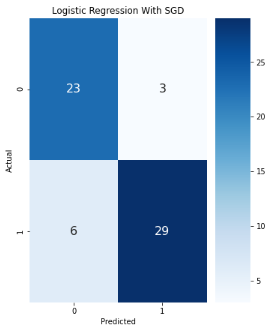
\includegraphics[scale=0.5]{Images/logCONFUSION.png}
    \end{center}
    \caption{Confusion matrix for the baseline logistic regression model}
\end{figure}

We can interpret the confusion matrix as follows:
\begin{itemize}
    \item \textbf{Top Left TP: } These are the true positive values, a person with a heart disease was correctly classified as a person who has a heart disease.
    \item \textbf{Top Right FP: } These are the false positives. A person with a healthy heart was incorrectly classified as a person who has a heart disease.
    \item \textbf{Bottom Left FN: } These are false negatives. False negatives are people that have been classified as not having any heart diseases when they actually do have heart diseases. This is a worst-case scenario and we want this value to be as low as possible.
    \item \textbf{Bottom Right TN: } True negatives are those people who are correctly classified as not having any heart diseases.
\end{itemize}

The accuracy of this model can be calculated as the $\frac{TN + TP}{TP + TN + FP + FN}$ which gives an accuracy of approximately $75\%$

Another thing worth noting is the graph that shows the error from the time of training to the end of training. This graph shows us that over time we were able to minimize the error. Take a good look at the graph below.
\begin{figure}[H]
    \begin{center}
        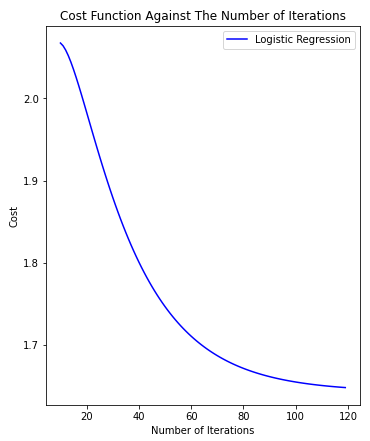
\includegraphics[scale=0.5]{Images/logCOST.png}
    \end{center}
    \caption{Cost function over a number of iterations for a baseline logistic regression implementation}
\end{figure}

One last figure we would like to discuss in this subsection is the ROC curve. The ROC curve basically gives us a visual presentation of how good our model is. If the curve is on the far left, this means the model is good, if it leans towards a straight line, then our model can not be relied upon.
\begin{figure}[H]
    \begin{center}
        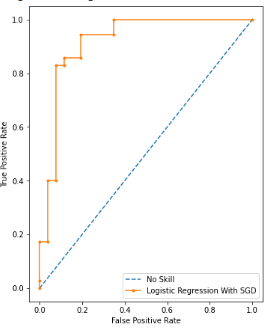
\includegraphics[scale=0.5]{Images/logROC.png}
    \end{center}
    \caption{ROC curve for a baseline logistic regression implementation}
\end{figure}
We can conclude this subsection with a comment regarding the ROC curve. Clearly, our model, though it has not been optimized looks to be doing a good job.


\section{Optimization Techniques}
In this chapter, we discuss the optimization techniques we have employed. These techniques were employed in making our original model better. We mainly aim to get better accuracies with our results, but these optimization techniques optimize other things other than improving accuracy. Optimization techniques can optimize the training time, data quality, etc.

\subsection{Employed techniques}
We hoped we could have more time to explore many more ways of optimizing logistic regression. We however only considered two optimization techniques, these are:

\subsubsection{Regularization}
Sometimes we have a complex model that aims to solve an easy problem. For instance, we could have a model that aims to solve a problem of a cubic function only to find that our data takes a linear shape. This leads to overfitting. Regularization aims to avoid overfitting by penalizing higher-order polynomials so that they have minimal effect on our overall model. We achieve regularization by adding a regularization term to our cost function. Our cost function will then take the shape below.
\begin{equation}
    J(\theta) = -\frac{1}{m}\sum_{i=1}^{n}[y^{(i)}log(h_{\theta}(x^{(i)})) + (1-y^{(i)})log(1-h_{\theta}(x^{(i)}))] +\frac{\lambda}{2m}\sum_{j=1}^m \theta_j^2 
\end{equation}

where $\lambda$ determines how much should we penalize $\theta$

To find $\theta's$ that minimizes the cost function, we have the following derivative:
\begin{equation}
    \frac{\partial}{\partial \theta_j}J(\theta) = \frac{1}{m}[ \sum_{i=1}^n(h(x^{(i)}) - y^{(i)})x_j^{(i)} + \lambda \theta_j ] 
\end{equation}
Gradient descent remains the same except that except that we replace the derivative with the new derivative above.

In our implementation, we train and the regularized logistic regression on two different datasets. We train on the dataset which had the missing values dropped and the datasets which had the missing values replaced with the mode in that particular column. We will then compare the results and make conclusions thereof.


\subsubsection{Mini-Batch Gradient Descent}
Before we explain what Mini-Batch gradient descent is, we first need to explain what other gradient descents exist and why have we chosen this approach. At this point of the report, we believe you as a reader know how gradient descent work from an abstract point of view. We therefore only going to focus on the differences of these gradient descents. There are three types of gradient descents, namely:
\begin{itemize}
    \item \textbf{Batch: }Batch gradient descent aims to take a single step only upon considering all records in the datasets and takes the average gradient of all data points in the training set. The problem arises when the dataset is too large. If the dataset is too large, then we could take forever to train a simple model. Batch gradient descent is great for convex functions.
    \item \textbf{Stochastic: }Stochastic gradient descent is the one we have used in our baseline implementation. Stochastic gradient descent poses a problem with not reaching the minimum due to the costs decreasing with fluctuations. SGD is great for datasets of large sizes.
    \item \textbf{Mini-Batch: }Mini-Batch is a mixture of both Bath and SGD. It aims to tackle problems that arise with using either Batch or SGD. Stochastic is more computationally expensive while Batch converges directly to a minimum. The idea here is that we want to converge faster while minimizing computational expense.
\end{itemize}

We have implemented Mini-Batch gradient descent in an attempt to optimize both computational expense and accuracy. We, however, only run the Mini-Batch on one dataset even though we have two, which we discussed in the previous subsection. We also did not implement Mini-Batch gradient descent with regularized logistic regression.  The reason for missing some implementation is due to the constraints of time.

\subsection{Outcomes of optizimations}

\newpage
\section{Conclusion}

